\documentclass[a4paper,12pt]{article}
\usepackage[utf8]{inputenc}
\usepackage[T1]{fontenc}
\usepackage[spanish]{babel}
\usepackage{csquotes}
\usepackage{anysize}
\usepackage{graphicx}
\marginsize{25mm}{25mm}{25mm}{25mm}

\title{Observer biases in the 3D interpretation of line drawings}
\author{Pascal Mamassian \and Michael S. Landy}
\date{1998}

\begin{document}
{\scshape\bfseries \maketitle}

{\scshape\bfseries Introducción}

Varias claves visuales permiten estimar la estructura tridimensional del ambiente, como la profundidad, orientación, forma, disparidad binocular, o movimiento relativo. Cada pista habla de un único atributo del ambiente. Pero dada la cantidad limitada de información, las computaciones que se hacen con estas pistas están poco delimitadas, es decir, que hay más de una solución posible. 

Se puede resolver este problema de dos maneras: usar otras claves para llenar los ``espacios vacíos'' que deja una ({\itshape e.g.,} el paralaje de movimiento complementa a la disparidad ocular al dar un estimado de la profundidad). La otra manera sería imponer presunciones a priori en los parámetros faltantes. Un ejemplo en el que este conocimiento es crítico es en la interpretación de imágenes simples. En ellas, las claves pictóricas indican una escena en 3D, pero la falta de disparidad ocular y de paralaje de movimiento indican una imagen plana.

A pesar de la ambigüedad en este tipo de imágenes los humanos tienen interpretaciones sumamente robustas.

{\scshape Shape-from-contour}

Las líneas en las imágenes pueden tener muchos orígenes, como cambios en la forma tridimensional, en figura-fondo, y en la reflectividad o iluminación. Estos últimos, llamados contornos de superficie ({\itshape surface contours}) son especialmente ambiguos, por lo que la estimación de la forma con base en los contornos de superficie ({\itshape shape-from-contour}) es fundamentalmente distinta de la estimación de la forma con base en marcas de textura ({\itshape shape-from-texture}).

Hay un número infinito de contornos tridimensionales que pueden dar lugar a un contorno de imagen. Para resolver este problema Stevens propuso que un observador hace tres suposiciones previas: 

\begin{enumerate}
	\item Los contornos de superficie son líneas de curvatura: las líneas de curvatura son las direcciones en una superficie sobre las cuales la orientación local cambia en el grado mayor y menor ({\itshape e.g.,} en un cilindro estas líneas son paralelas a los meridianos).
	\item Los contornos de superficie son geodésicos: las curvas geodésicas en una superficie son generalizaciones de líneas rectar en un plano. Su curvatura se debe solamente a la curvatura de la superficie.
	\item El objeto y el observador están en posición general: esta presunción limita las posibles interpretaciones de una escena de modo que, por ejemplo, un contorno recta en una imagen nunca sea interpretado como un contorno tridimensional curvado.
\end{enumerate}

{\scshape Overview}

Se tomará una aproximación psicofísica y computacional para encontrar las presunciones que los observadores usan para entender dibujos. Se usarán imágenes compuestas por dos grupos de contornos paralelos ambiguos que pueden parecer cóncavos o convexos. Las interpretaciones ocurren con mayor o menor frecuencia de acuerdo con sesgos. Los sesgos se miden con ayuda de un modelo estocástico que sabe sobre la geometría de la formación de imágenes e incorpora limitaciones explícitas en forma de priors. Es una instancia simple de modelo Bayesiano.

{\scshape\bfseries Human observers' biases}

En estos dibujos la forma sólida es un continuo del que emergen dos categorías: la forma elíptica y la forma hiperbólica. Se pidió a los observadores ver imágenes como la figura 1 y categorizarlas como elípticas o hiperbólicas. 

\begin{figure}[hb]
	\begin{center}
		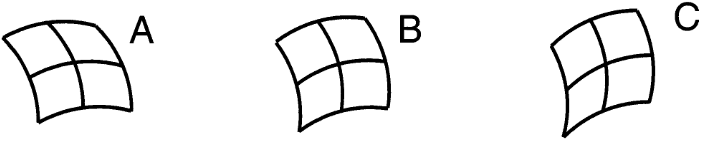
\includegraphics[scale=0.5]{Mamassian1998(1).png}
		\caption{Ejemplos de estímulos usados en la tarea}
	\end{center}
\end{figure}

{\scshape Methods}

Los estímulos estaban formados de seis arcos circulares idénticos acomodados en dos sets de contornos paralelos. Tres figuras fueron usadas: la figura A estaba comprimida en su eje de simetría, mientras que la C estaba estirada sobre su eje. La figura B era un punto intermedio entre ambas. Las elongaciones eran tales que la intersección central de A, B, y C formaba ángulos de 75, 90 y 105°. 

{\scshape Procedure}

Se usó un paradigma de elección forzada. En cada ensayo los observadores miraban una figura y reportaban en un teclado si su primera impresión era elíptica o hiperbólica. La figura se mostraba en una orientación aleatoria en pasos de 15°. Se mostraban las 3 figuras en las 24 orientaciones posibles en orden aleatorio. La visión era monocular por tiempo ilimitado.

{\scshape Results and discussion}

El {\itshape aspect ratio} de la figura (si se trataba de A, B o C) tuvo un gran impacto en la proporción de veces que fue percibida como {\itshape con forma de huevo} (``{\itshape elliptic score}''). La forma A, comprimida en su eje de simetría, fue percibida más a menudo como con forma de huevo en todas sus orientaciones (alto {\itshape elliptic score}), mientras que la forma C fue más a menudo percibida como con forma de silla de montar en todas sus orientaciones (bajo {\itshape elliptic score}). La forma B fue percibida distinto dependiendo de su orientación: cuando su eje de simetría era cercano a vertical, se percibía como elíptica. Cuando era cercano a horizontal, era percibida como hiperbólica.

Una potencial explicación para la dependencia de la orientación es que los observadores interpretan aquellos contornos que son convexos hacia arriba como si se originaran de marcas convexas en la superficie del objeto. Cuando dos contornos se intersecan en una imagen, el dibujo es interpretado como elíptico si los dos contornos son cóncavos o convexos, e hiperbólica si uno es cóncavo y el otro convexo. El efecto de la orientación de la imagen se predice dado que los contornos convexos se vuelven cóncavos (y viceversa) cuando la imagen es rotada 180°. La correspondencia entre convexidad de la imagen y convexidad de la superficie es una presunción de que la superficie está orientada de forma tal que su normal apunta hacia arriba, como si el observador mirara hacia abajo.

Es importante notar que el cambio en interpretación de elíptica a hiperbólica en la figura B es gradual. Un modelo que explique los datos debe reflejar esta propiedad. La aproximación de los autores es la definición de un ``observador Bayesiano simple''.

{\scshape\bfseries Simple Bayesian observer}

Dado un dibujo se quiere predecir la probabilidad de que los sujetos perciban la superficie como elíptica. Dado que se involucran sesgos, es natural adoptar una aproximación Bayesiana. 

{\scshape Model construction}

{\itshape Rationale}

Dado que los observadores se sesgan a una u otra interpretación para un dibujo dado se infiera que usan suposiciones sobre la imagen. Un análisis Bayesiano incluye estas suposiciones en el proceso de inferencia.

Un modelo de esta naturaleza se compone de dos etapas: primero las suposiciones se codifican como distribuciones de probabilidad de priors, que luego se combinan con la información de la imagen usando la regla de Bayes. Esto llevará a la probabilidad de que una superficie sea elíptica para una imagen dada (la probabilidad posterior). La segunda parte del modelo convierte la probabilidad posterior en una respuesta según una regla de decisión.

Por simplicidad se considerará solamente la intersección central de los dibujos. Tampoco se considerará la curvatura de los contornos dado que se mantuvo constante. Así, para cada dibujo se mide la orientación de cada una de las curvas en su punto de intersección, y la orientación se codifica de forma relativa a la normal de las curvas. Así, las dos orientaciones $\varphi_{1}$ y $\varphi_{2}$ están entre 0 y $\pi$ si la curva es localmente convexa hacia arriba, y entre $\pi$ y $2\pi$ si es convexa hacia abajo. Así, la probabilidad posterior a computar por la primera parte del modelo es 
\begin{equation}
	P(elliptic | \varphi_{1}, \varphi_{2}),
\end{equation}
es decir, la probabilidad de que la superficie sea elíptica dada la orientación de las dos curvas.

Para computar esta probabilidad se debe estimar la verosimilitud de que cierta escena dé lugar a los datos de la imagen (descritos por $\varpi_{1}$ y $\varpi_{2}$), y modelar la probabilidad previa para cada escena (antes de haber mirado la imagen).

La escena se caracteriza por tres factores: (1) la orientación del parche relativa al observador, (2) la forma local al centro del parche, y (3) la orientación de las marcas de superficie en el parche. Se proveerá un modelo estocástico (en forma de una distribución prior) parametrizado para cada uno de los factores. Específicamente se caracterizará una preferencia por percibir una superficie (1) orientada con sus puntos normales hacia arriba, (2) localmente convexa, y (3) con contornos de imagen alineados con las líneas principales de curvatura. Estos tres sesgos permiten explicar los resultados.

Se asumirá que la orientación, forma y orientación de marcas de superficie constituyen eventos independientes de modo que la probabilidad posterior puede derivarse simplemente mediante la regla de Bayes. Después se elegirá una regla de decisión para mapear la probabilidad posterior en un {\itshape elliptic score}.

A continuación se derivarán las tres distribuciones prior, se computará la verosimilitud para el problema, y se combinarán las tres distribuciones usando la regla de Bayes.

{\scshape Surface orientation prior distribution}

La orientación puede representarse con tres ángulos: tilt $\tau$, slant $\sigma$, y roll $\rho$ (Figura 2).

\begin{figure}[hb]
	\begin{center}
		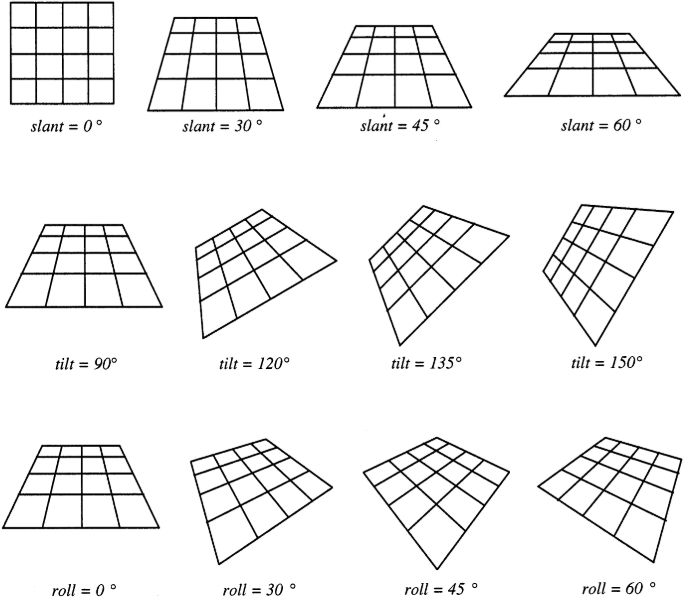
\includegraphics[scale=0.5]{Mamassian1998(2).png}
		\caption{Ángulos que representan la orientación.}
	\end{center}
\end{figure}

Se propondrán distribuciones de priors para $\tau$, $\sigma$ y $\rho$.

Si un observador no tiene sesgo en el tilt, la imagen debería interpretarse siempre de la misma forma sin importar su orientación en el plano frontal, pero se ha encontrado que no es así. Cuando las superficies son más o menos horizontales, este sesgo toma una forma intuitiva: las superficies son más frecuentemente vistas desde arriba que desde abajo. Por lo tanto se incluirá un sesgo en el tilt de la superficie en la orientación hacia arriba $\frac{\pi}{2}$. Se asume una distribución Gaussiana:
\begin{equation}
	P(\tau)
	=
	\frac{
		1
	}{
	\sqrt{2\pi \sigma_{\tau}}
	}
	\mbox{exp}
	\left(
		-\frac{
			(\tau-\frac{\pi}{2})^{2}
		}{
			2\sigma_{\tau}^{2}
		}\right).
\end{equation}

La desviación estándar $\sigma_{\tau}$ de la distribución Gaussiana controla el grado del sesgo. Un valor de $\infty$ corresponde a la ausencia de sesgo se la dirección de observación.

No hay evidencia de sesgos que correspondan al slant, por lo que se asumirá la ausencia de ellos. Es decir, se asume una distribución que resultaría en una distribución uniforme de orientaciones de superficie si el tilt también fuese insesgado. La distribución es, entonces,
\begin{equation}
	P(\sigma) = sin(\sigma)
\end{equation}

Tampoco hay evidencia de sesgos para el roll, por lo que se asumirá una distribución sin sesgo. Se restringirá la distribución de $\rho$ a una uniforme entre 0 y $\frac{\pi}{2}$.

Asumiendo que los componentes son independientes, se puede obtener la probabilidad conjunta $P(\tau,\,\sigma,\,\rho)$ del producto de las probabilidades individuales.

{\scshape Local shape prior distribution}

La forma sólida se puede resumir por dos parámetros nombrados {\itshape shape characteristic} y {\itshape curvature magnitude}. Shape characteristic $\chi$ indica si la superficie es localmente elíptica ($0<\chi<1$) o localmente hiperbólica ($-1\leq \chi< 0$), mientras la curvature magnitude $\eta$ indica si la superficie es localmente convexa ($\eta>0$) o cóncava ($\eta<0$).

Se preguntó a los sujetos si la figura era elíptica o hiperbólica. Lo cóncavo/convexo era irrelevante. Sin embargo, hay evidencia que indica que superficies cóncavas y convexas no son tratadas igualmente: en esta misma tarea la figura A rotada 0 y 180° era percibida como convexa y cóncava, y ambos casos mostraron diferencias en el {\itshape elliptic score}.

Para integrar las diferencias en entre superficies cóncavas y convexas en el modelo se integra un sesgo en la curvature magnitude, que es proporcional a una de las curvaturas principales $k$. Se eligió de nuevo una distribución Gaussiana para la distribución de este sesgo:
\begin{equation}
	P(k_{i})
	=
	\frac{
		1
	}{
	\sqrt{2\pi}
	}
	\mbox{exp}
	\left(
		-
		\frac{
		k_{i}-\mu_{k}
		}{
			2
		}
	\right)^{2},\ \ i=1,2.
\end{equation}

Por simplificar solo se presta atención al signo de la curvatura de la imagen en la intersección de las líneas, y no a el grado mismo de la curvatura. 

{\scshape Surface marking orientation prior distribution}

Un cambio muy pequeño en el {\itshape aspect ratio} de la figura produce un gran sesgo en la percepción. Esto fue difícil de reproducir en el modelo. Para esto se explotó la forma en que las marcas de superficie se organizan en el parche tridimensional. Primero se intentó favorecer configuraciones en las cuales los contornos fueran geodésicos y ortogonales entre sí. Pero este sesgo no fue suficiente para explicar el gran cambio en la forma percibida. Así, se integró la presunción de que las marcas de superficie están orientadas aproximadamente siguiendo las direcciones principales. De nuevo se escogió una distribución Gaussiana. $\psi$ denota la orientación de una marca de superficie tangente al plano relativo a la primera dirección principal:

\begin{equation}
\left\{
	\begin{array}{l}
		P(\psi_{1})
		=
		\frac{
			1
		}{
		\sqrt{2\pi}\sigma_{\psi}
		}
		\mbox{exp}
		\left(
		-\frac{
			\psi_{1}-\rho
		}{
			2\sigma^{2}_{\psi}
		}
		\right)^{2}
		
		\\

		P(\psi_{2})
		=
		\frac{
			1
		}{
		\sqrt{2\pi}\sigma_{\psi}
		}
		\mbox{exp}
		\left(
		-\frac{
			\psi_{2} - \rho - \frac{\pi}{2}
		}{
			2\sigma_{\psi}^{2}
		}
		\right)^{2}.
	\end{array}	
\right.
\end{equation}

La desviación estándar $\sigma$ controla la fuerza del sesgo. Y aunque las dos direcciones principales son ortogonales y por lo tanto no independientes, se puede computar la probabilidad conjunta $P(\psi_{1},\, \psi_{2})$.

{\scshape Bayesian combination}

Se ha caracterizado la escena en términos de su orientación ($\tau$, $\sigma$ y $\rho$), forma local de superficie ($\eta$ y $\chi$), y marcas de suuperficie ($\psi_{1}$ y $\psi_{2}$). El modelo computa las probabilidades posteriores en términos de esas variables dadas las orientaciones de imagen $\varphi_{1}$ y $\varphi_{2}$. La probabilidad posterior puede expandirse como
\begin{equation}
		P(elliptic | \varphi_{1}, \varphi_{2})
		=
		\int_{\Omega}
		P(\tau,\sigma,\rho,\chi,\eta,\psi_{1},\psi_{2} | \varphi_{1}, \varphi_{2})
		\times
		d\tau\, d\sigma\, d\rho\, d\chi\, d\eta\, d\psi_{1}\, d\psi_{2}.
\end{equation}

La integración tiene lugar en el dominio $\Omega$, que es el producto de los dominios de orientación de superficie, forma de superficie, y orientación de marcas de superficie.

Usando la regla de Bayes se puede reescribir el integrando como
\begin{equation}
	\frac{
		P(
			\varphi_{1},\varphi_{2}
			|
			\tau,\sigma,\rho,\chi,\eta,\psi_{1},\psi_{2}
		)
		P(
		\tau,\sigma,\rho
		)
		P(
			\chi,\eta
		)
		P(
		\psi_{1},\psi_{2}
		)
	}{
	P(\varphi_{1}, \varphi_{2})
	}
\end{equation}

{\scshape Likelihood}

En la ecuación anterior el primer término del numerador es la verosimilitud. Representa el proceso de formación de la imagen: ¿es la imagen (más bien la intersección de las líneas en el centro) compatible con la proyección de una escena tridimensional particular? Si la formación de la imagen está libre de ruido (si la proyección de un objeto a un plano está únicamente determinada) entonces esta verosimilitud es una función delta
\begin{equation}
	\begin{array}{l}
		P(\varphi_{1}, \varphi_{2} | \tau,\sigma,\rho,\chi,\eta,\psi_{1},\psi_{2})
		=\\
		\left\{
		\begin{array}{l}
			1,\,if\,\varphi_{1} = F(\tau,\sigma,\rho,\chi,\eta,\psi_{1})\,and\,\varphi_{2} = F(\tau,\sigma,\rho,\chi,\eta,\psi_{2})\\
			0\,\ otherwise
		\end{array}
		\right.
	\end{array}
\end{equation}

Donde $F(\tau,\sigma,\rho,\chi,\eta,\psi)$ es la función que proyecta una curva con orientación $\psi$ en la superficie en una curva con orientación $\varphi$ en la imagen. Sin meterse en la geometría, se obtiene que
\begin{equation}
	F(\tau,\sigma,\rho,\chi,\eta,\psi)
	=
	\arctan\left(
		\frac{
			\tan(\psi + \rho)
		}{
		\cos(\sigma)
		}
	\right)
	+
	\mbox{sign}(k\,\tan(\psi + \rho)) \frac{\pi}{2} + \tau
\end{equation}
donde $k$ es la curvatura de la marca de superficie en la intersección de las líneas.

{\scshape Decision rule}

Una elección popular es {\itshape maximum a posteriori} (MAP), en la cual el observador elige la interpretación con la mayor probabilidad posterior, lo que minimiza el número de errores esperados. Sin embargo, en este caso no hay una señal de realimentación tras la decisión del sujeto, por lo que no se justifica usar esa regla. Se puede decir que los observadores enfrentan un problema de inferencia estadística pura en el que simplemente deben dar un resumen de la evidencia estadística para la forma local estimada. Por lo tanto, tiene sentido que los juicios de los observadores reflejen directamente la probabilidad posterior:
\begin{equation}
	P(\mbox{Observer responds `elliptic'|image}) = P(\mbox{Surface shape is `elliptic'|image})
\end{equation}

Dado que la probabilidad del juicio es igual a la probabilidad posterior este modelo es llamado ``modelo Bayesiano simple''. Una diferencia clave con otros modelos con reglas de decisión más clásicas es que no se necesita de una fuente de ruido para que los juicios sean probabilísticos.

{\scshape Results}

Se utilizó el método de Monte Carlo para muestrear probabilidades de priors y construir la probabilidad posterior. El modelo tiene tres parámetros que controlan la fuerza de cada uno de los sesgos. Estos parámetros se ajustaron para obtener el ajuste de mayor verosimilitud a los datos. El ajuste se muestra en la figura 3.

\begin{figure}[hb]
\begin{center}
	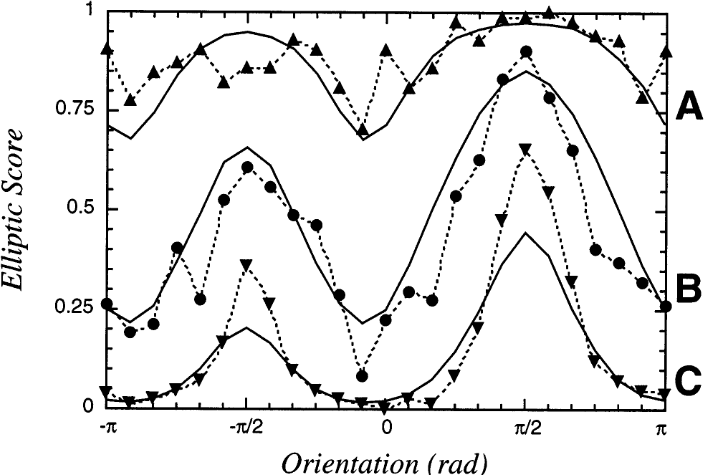
\includegraphics[scale=0.5]{Mamassian1998(3).png}
	\caption{Ajuste del modelo con los datos de los tres estímulos.}
\end{center}
\end{figure}

Se creó un modelo alternativo en el cual se impuso una limitación en la orientación de las marcas de superficie de modo que éstas fueran simplemente geodésicas y aproximadamente ortogonales en lugar de aproximadamente alineadas con las direcciones principales. El modelo modificado tuvo un ajuste significativamente peor con los datos.

Del mismo modo se probaron modelos reducidos en los que se eliminó alguno de los sesgos. Para esto se ajustó alguno de los tres parámetros para que su sesgo asociado fuese eliminado. Los parámetros restantes fueron estimados de nuevo por máxima verosimilitud. Se encontró que la eliminación de cualquiera de los sesgos disminuía en gran medida el ajuste con los datos, y que cada sesgo era requerido para que el modelo capturara alguna característica importante en los datos: el sesgo en la orientación de superficie ($\sigma_{\tau}$) se requiere para que la orientación tenga efecto sobre la forma percibida; el sesgo en la orientación de las marcas de superficie ($\sigma_{\psi}$) es responsable de las diferencias en percepción entre las tres formas; y el sesgo en la forma de superficie ($\mu_{k}$) es responsable de las asimetrías en los juicios dados a rotaciones de 180° en las imágenes.

{\scshape\bfseries Discussion}

A pesar de que había un número infinito de curvas tridimensionales que podían proyectar los dibujos, los observadores tendían a percibir solamente una de dos formas básicas: elípticas o hiperbólicas. La percepción de una u otra forma dependía no solo de la geometría del dibujo, sino de su orientación también. Los resultados no son acordes con un mundo en el que es igualmente probable que los parches ocurran en cualquier orientación, con cualquier forma y con cualesquiera marcas de superficie. En lugar de ello los sujetos mostraron sesgos consistentes. El análisis de la frecuencia de las respuestas permitió observar estos sesgos, que fueron después formalizados en un modelo Bayesiano simple. Los sesgos fueron modelados en forma de funciones de probabilidad prior, y la regla de decisión fue {\itshape non-committing}, es decir, se igualó la probabilidad de respuesta con la probabilidad posterior.

Por conveniencia matemática se asumió que todos los contornos de superficie eran geodésicos, es decir, que la curvatura de un contorno de superficie se debe solamente a la curvatura de la superficie. Relajar esta limitación implicaría que una porción de la curvatura de la imagen podría ser independiente de la geometría de la superficie, como un tipo de ruido.

En este modelo, dado que la curvatura de los contornos era constante, el grado de curvatura se ignoró y sólo se tomó en cuenta su signo. Aunque sería posible e interesante elaborar un modelo que incluyera la magnitud de la curvatura.

Cabe preguntarse cuán fuertes son los sesgos incluidos y cuanta confianza pone en ellos el sistema visual. Cualquiera de los sesgos puede violarse, pero permiten dar una buena primera impresión sobre el estado del mundo que se puede corregir más adelante cuando se obtiene más información.

Presumiblemente {\itshape shape-form-contour} no es la única clave que se basa en suposiciones a priori. En otras situaciones en que distintas claves no pueden interactuar para llenar la información faltante, los observadores necesitan de las presunciones.

\end{document}
